\documentclass[paper=letter, fontsize=11pt]{scrartcl} 
 \usepackage[top=2.5cm, bottom=2.5cm, left=2.5cm, right=2.5cm]{geometry}
\usepackage{framed}

\usepackage{graphicx}
\usepackage{verbatim}
\usepackage{pictex}  
\usepackage{multimedia}
\usepackage{listings}
\usepackage{xcolor,colortbl}
\usepackage[spanish]{babel} % language/hyphenation
\usepackage{amsmath,amsfonts,amsthm} % Math packages
\usepackage{amsbsy}
\usepackage{amssymb}
\usepackage{fancyvrb}
\usepackage{sectsty} % Allows customizing section commands
\usepackage[dvipsnames]{xcolor}

\newcommand{\defi}[3]{\textbf{Definición:#3}}
\newcommand{\fin}{$\blacksquare.$}
\newcommand{\finf}{\blacksquare.}

\newcommand{\grstep}[2][\relax]{%
   \ensuremath{\mathrel{
       {\mathop{\longrightarrow}\limits^{#2\mathstrut}_{
                                     \begin{subarray}{l} #1 \end{subarray}}}}}}
\newcommand{\swap}{\leftrightarrow}

\newcommand{\gen}{\text{gen}}

\newtheorem{thmt}{Teorema:}
\newtheorem{thmd}{Definición:}
\newtheorem{thml}{Lema:}
\newtheorem{thmj}{Ejemplo:}
\newtheorem{thma}{Algoritmo:}
\newtheorem{thmp}{Propiedad:}


\newcommand{\mub}{\mathbf{\mu}}
\newcommand{\Sb}{\mathbf{S}}
\newcommand{\mb}{\mathbf{m}}
\newcommand{\cb}{\mathbf{c}}
\newcommand{\xb}{\mathbf{x}}
\newcommand{\Xb}{\mathbf{X}}
\newcommand{\yb}{\mathbf{y}}
\newcommand{\Yb}{\mathbf{Y}}
\newcommand{\Simgab}{\mathbf{\Sigma}}
\newcommand{\sumk}{\sum_{k=1}^K}
\newcommand{\sumi}{\sum_{i=1}^n}
\newcommand{\sumj}{\sum_{j=1}^n}
\usepackage{biblatex}
\addbibresource{biblio.bib}

\allsectionsfont{\centering \normalfont\scshape} % Make all sections centered, the default font and small caps
\usepackage{float}
\usepackage{fancyhdr} % Custom headers and footers
\pagestyle{fancyplain} % Makes all pages in the document conform to the custom headers and footers
\fancyhead{} % No page header - if you want one, create it in the same way as the footers below
\fancyfoot[L]{} % Empty left footer
\fancyfoot[C]{} % Empty center footer
\fancyfoot[R]{\thepage} % Page numbering for right footer
\renewcommand{\headrulewidth}{0pt} % Remove header underlines
\renewcommand{\footrulewidth}{0pt} % Remove footer underlines
\setlength{\headheight}{13.6pt} % Customize the height of the header
\usepackage{biblatex}
\addbibresource{references.bib}
\numberwithin{equation}{section} % Number equations within sections (i.e. 1.1, 1.2, 2.1, 2.2 instead of 1, 2, 3, 4)
\numberwithin{figure}{section} % Number figures within sections (i.e. 1.1, 1.2, 2.1, 2.2 instead of 1, 2, 3, 4)
\numberwithin{table}{section} % Number tables within sections (i.e. 1.1, 1.2, 2.1, 2.2 instead of 1, 2, 3, 4)

\setlength\parindent{0pt} % Removes all indentation from paragraphs - comment this line for an assignment with lots of text

\newcommand{\horrule}[1]{\rule{\linewidth}{#1}} % Create horizontal rule command with 1 argument of height

\title{	
\normalfont \normalsize 
\textsc{Centro de Investigaci\'on en Matem\'aticas (CIMAT). Unidad Monterrey} 
\\ [25pt] 
\horrule{0.5pt} \\[0.4cm] % Thin top horizontal rule
\huge Tarea 5 \\ 
\horrule{2pt} \\[0.5cm] % Thick bottom horizontal rule
}


\author{Enrique Santibáñez Cortés} % Your name

\date{\normalsize\today} % Today's date or a custom date

\begin{document}
\lstdefinestyle{customc}{
  belowcaptionskip=1\baselineskip,
  basicstyle=\footnotesize, 
  frame=lrtb,
  breaklines=true,
  %frame=L,
  %xleftmargin=\parindent,
  language=C,
  showstringspaces=false,
  basicstyle=\footnotesize\ttfamily,
  keywordstyle=\bfseries\color{green!40!black},
  commentstyle=\itshape\color{red!40!black},
  identifierstyle=\color{blue},
  stringstyle=\color{purple},
}

\lstset{breakatwhitespace=true,
  basicstyle=\footnotesize, 
  commentstyle=\color{green},
  keywordstyle=\color{blue},
  stringstyle=\color{purple},
  language=C++,
  columns=fullflexible,
  keepspaces=true,
  breaklines=true,
  tabsize=3, 
  showstringspaces=false,
  extendedchars=true}

\lstset{ %
  language=R,    
  basicstyle=\footnotesize, 
  numbers=left,             
  numberstyle=\tiny\color{gray}, 
  stepnumber=1,              
  numbersep=5pt,             
  backgroundcolor=\color{white},
  showspaces=false,             
  showstringspaces=false,       
  showtabs=false,               
  frame=single,                 
  rulecolor=\color{black},      
  tabsize=2,                  
  captionpos=b,               
  breaklines=true,            
  breakatwhitespace=false,    
  title=\lstname,             
  keywordstyle=\color{blue},  
  commentstyle=\color{dkgreen},
  stringstyle=\color{mauve},   
  escapeinside={\%*}{*)},      
  morekeywords={*,...}         
} 

\maketitle

\section{Clasificación binaria}

\subsection{Introducción}
Para datos de clasificación binaria $\{(\xb_i, Y_i)\}_{i=1}^n$, consideremos la siguiente función de costo
\begin{align}\label{costo}
    L=\sumi\left(\theta(y_i)-\beta'\xb_i-\beta_0 \right)^2
\end{align}
Definamos $n_+, n_-$ el número de observaciones con $y_i=1$ y $y_i=-1,$ respectívamente $\cb_+, \cb_-$ el centroide de las observaciones con $y_i=1,$ y $y_1=-1$ y $\cb$ el centroide de todos los datos. Y definamos las siguientes matrices:

\begin{align} \label{d_matrices}
    \Sb_B &= (\cb_+-\cb_-)(\cb_+-\cb_-)'\\
    \Sb_W &=\sum_{i:y_i=1}(\xb_i-\cb_+)(\xb_i-\cb_+)'+\sum_{i:y_i=-11}(\xb_i-\cb_-)(\xb_i-\cb_-)'
\end{align}

\subsection{Propiedades de las matrices $\Sb_B$ y $\Sb_W$}
\begin{framed}
    \begin{thmp} 
    \label{a_kernel}
    $$\Sb_w=\sum_{i:y_i=1}\xb_i\xb_i'+\sum_{i:y_i=-1}\xb_i\xb_i'-n_{+}\cb_{+}\cb_{+}'-n_{-}\cb_{-}\cb_{-}'$$
    \end{thmp}
\end{framed}

\textbf{Demostración de la Propiedad: 1.} Recordemos que $\cb_{+}=\frac{1}{n_+}\sum_{i:y_i=1}x_i$ y $\cb_{-}=\frac{1}{n_-}\sum_{i:y_i=-1}x_i$. Ahora simplemente desarrollamos los productos de la definición de $\Sb_W$ (\ref{d_matrices}),
\begin{align*}
    \Sb_W &=\sum_{i:y_i=1}(\xb_i-\cb_+)(\xb_i-\cb_+)'+\sum_{i:y_i=-11}(\xb_i-\cb_-)(\xb_i-\cb_-)'
\end{align*}
\begin{align*}
\ \ \ \ \ \ &= \sum_{i:y_i=1}\left(\xb_i\xb_i'-2\cb_+\xb_i'+\cb_+\cb_+'\right)+\sum_{i:y_i=-1}\left(\xb_i\xb_i'-2\cb_-\xb_i'-\cb_-\cb_-'\right)\\
    &=\sum_{i:y_i=1}\xb_i\xb_i'-2\cb_+\sum_{i:y_i=1}\xb_i'+n_+\cb_+\cb_+'+\sum_{i:y_i=-1}\xb_i\xb_i'-2\cb_-\sum_{i:y_i=-1}x_i'-n_-\cb_-\cb_-'\\
    &=\sum_{i:y_i=1}\xb_i\xb_i'-2\cb_+(n_+\cb_+')+n_+\cb_+\cb_+'+\sum_{i:y_i=-1}\xb_i\xb_i'-2\cb_-(n_-\cb_-)-n_-\cb_-\cb_-'\\
    &= \sum_{i:y_i=1}\xb_i\xb_i'+\sum_{i:y_i=-1}\xb_i\xb_i'-n_+\cb_+\cb_+'-n_-\cb_-\cb_-' \ \finf
\end{align*}
\begin{framed}
    \begin{thmp} 
    \label{sb}
    El vector $\Sb_B\beta$ es un múltiplo del vector $(\cb_+-\cb_-).$
    \end{thmp}
\end{framed}
\textbf{Demostración de la Propiedad: 2.} Podemos definir a $\mb_+=\frac{1}{n_+}\sum_{i:y_i=1}\beta'x_i$ y $\mb_-=\frac{1}{n_-}\sum_{i:y_i=-1}\beta'x_i$, ya que son productos puntos de dos vectores podemos decir que $\mb_+$ y $\mb_-$ son escalares. Entonces ocupando la definición de $\Sb$, tenemos que
\begin{align*}
   \Sb_B\beta&= (\cb_+-\cb_-)(\cb_+-\cb_-)'\beta=(\cb_+-\cb_-)(\cb_+\beta'-\cb_-\beta')'\\
   &=(\cb_+-\cb_-)\left(\frac{1}{n_+}\sum_{i:y_i=1}\beta'x_i-\frac{1}{n_-}\sum_{i:y_i=-1}\beta'x_i\right)'\\
   &=(\cb_+-\cb_-)(\mb_+-\mb_-)'=(\cb_+-\cb_-)\bf{\gamma},
\end{align*}
donde $\gamma=\left(\frac{1}{n_+}\sum_{i:y_i=1}\beta'x_i-\frac{1}{n_-}\sum_{i:y_i=-1}\beta'x_i\right)'.$ Por lo tanto, podemos decir que $\Sb_B\beta$ es un múltiplo del vector $(\cb_+-\cb_-)$ \ \ \fin
\begin{framed}
    \begin{thmp} 
    \label{sb}
    Sea $\theta(1)=\frac{n}{n_+}$ y $\theta(-1)=-\frac{n}{n_-}$, tenemos que el mínimo de (\ref{costo}) es
    \begin{align*}
        \beta_0&=-\beta'\cb.\\
        \left(\Sb_W+\frac{n_+n_-}{n}\Sb_B \right)\beta &=n(\cb_+-\cb_-).
    \end{align*}
    \end{thmp}
\end{framed}
\textbf{Demostración de la Propiedad: 3.} La función de costo se puede reescribir como
\begin{align*}
    \sumi\left(\theta(y_i)-\beta'\xb_i-\beta_0 \right)^2&=\sum_{i:y_i=1}\left( \theta(y_i)-\beta'\xb_i-\beta_0\right)^2+ \sum_{i:y_i=-1}\left( \theta(y_i)-\beta'\xb_i-\beta_0\right)^2\\
    &=\sum_{i:y_i=1}\left(\frac{n}{n_+}-\beta'\xb_i-\beta_0\right)^2+ \sum_{i:y_i=-1}\left(-\frac{n}{n_-}-\beta'\xb_i-\beta_0\right)^2.
\end{align*}
Ahora encontramos el mínimo de la expresión anterior para $\beta_0$, para ello primero derivamos respecto a $\beta_0$:
\begin{align*}
    \frac{\partial L}{\partial \beta_0}=-2\sum_{i:y_i=1}\left(\frac{n}{n_+}-\beta'\xb_i-\beta_0\right)-2\sum_{i:y_i=-1}\left(-\frac{n}{n_-}-\beta'\xb_i-\beta_0\right).
\end{align*}
Igualamos a cero la expresión anterior y despejamos a $\beta_0$,
\begin{align*}
    -2\sum_{i:y_i=1}\left(\frac{n}{n_+}-\beta'\xb_i-\beta_0\right)-2\sum_{i:y_i=-1}\left(-\frac{n}{n_-}-\beta'\xb_i-\beta_0\right)=&0\\
    \frac{nn_+}{n_+}-\beta'\sum_{i:y_i=1}\xb_i-n_+\beta_0-\frac{nn_-}{n_-}-\beta'\sum_{i:y_i=-1}\xb_i-n_-\beta_0=&0\\
    -\beta_0(n_++n_-)=&\beta'\left(\sum_{i:y_i=1}\xb_i+\sum_{i:y_i=-1}\xb_i\right)\\
    \beta_0 =& -\beta'\frac{1}{n}\sumi \xb_i\\
    \beta_0 =& -\beta' \cb \ \finf
\end{align*}
Realizando un procedimiento similar al anterior, derivamos la función de costo respecto a $\beta$
\begin{align*}
    \frac{\partial L}{\partial \beta} = -2\sum_{i:y_i=-1}\left( \frac{-n}{n_-} -\beta'\xb_i-\beta_0\right)\xb_i'-2\sum_{i:y_i=1}\left( \frac{n}{n_+} -\beta'\xb_i-\beta_0\right)\xb_i'.
\end{align*}
Ahora igualamos a cero e intentamos $\beta'$,
\begin{align*}
-2\sum_{i:y_i=1}\left( \frac{-n}{n_-} -\beta'\xb_i-\beta_0\right)\xb_i'-2\sum_{i:y_i=-1}\left( \frac{n}{n_+} -\beta'\xb_i-\beta_0\right)\xb_i'=&0\\
\frac{-n\sum_{i:y_i=-1}\xb_i}{n_-}-\beta'\sum_{i:y_i=-1}\xb_i \xb_i'-\beta_0\sum_{i:y_i=-1}\xb_i'+\frac{n\sum_{i:y_i=1}\xb_i}{n_+}-\beta'\sum_{i:y_i=1}\xb_i \xb_i'-\beta_0\sum_{i:y_i=1}\xb_i'&=0\\
-n\cb_--\beta'\sum_{i:y_i=-1}\xb_i \xb_i'-\beta_0\sum_{i:y_i=-1}\xb_i'+n\cb_+-\beta'\sum_{i:y_i=1}\xb_i \xb_i'-\beta_0\sum_{i:y_i=1}\xb_i'&=0\\
-\beta'\sum_{i:y_i=-1}\xb_i \xb_i'-\beta_0 n_- \cb_-'+-\beta'\sum_{i:y_i=1}\xb_i \xb_i'-\beta_0 n_+ \cb_+&=n\cb_--n\cb_+\\
-\beta'\sum_{i:y_i=-1}\xb_i \xb_i'+n_-\beta'\cb\cb_-'-\beta'\sum_{i:y_i=1}\xb_i \xb_i' +n_+\beta'\cb\cb_+'&=n(\cb_--\cb_+).
\end{align*}
Ocupando que $\cb=\frac{n_+\cb_++n_-\cb_-}{n}$ y $n=n_++n_-$, sustituimos en la expresión anterior
\begin{align*}
-\beta'\sum_{i:y_i=-1}\xb_i \xb_i'+n_-\beta'\cb\cb_-'-\beta'\sum_{i:y_i=1}\xb_i \xb_i' +n_+\beta'\cb\cb_+'&=n(\cb_--\cb_+)\\
-\beta'\sum_{i:y_i=-1}\xb_i \xb_i'+n_-\beta'\left( \frac{n_+\cb_++n_-\cb_-}{n}\right)\cb_-'-\beta'\sum_{i:y_i=1}\xb_i \xb_i' +n_+\beta'\left( \frac{n_+\cb_++n_-\cb_-}{n}\right)\cb_+'&=n(\cb_--\cb_+)\\
\left(\sum_{i:y_i=-1}\xb_i \xb_i'-\frac{n_-n_+\cb_+\cb_-'-n_-n_-\cb_-\cb_-'}{n}+\sum_{i:y_i=1}\xb_i \xb_i'-\frac{n_+n_+\cb_+\cb_+'-n_+n_-\cb_-\cb_+'}{n} \right)\beta&=n(\cb_+-\cb_-)\\
\left(\sum_{i:y_i=-1}\xb_i \xb_i'-\frac{n_-n_+\cb_+\cb_-'+n_-(n-n_+)\cb_-\cb_-'}{n}+\sum_{i:y_i=1}\xb_i \xb_i'-\frac{n_+(n-n_-)\cb_+\cb_+'-n_+n_-\cb_-\cb_+'}{n} \right)\beta&=n(\cb_+-\cb_-)\\
\left(\sum_{i:y_i=-1}\xb_i \xb_i'+\sum_{i:y_i=1}\xb_i \xb_i' +-n_-\cb_-\cb_-'-n_+\cb_+\cb_+'+\frac{n_-n_+}{n}\left(-\cb_+\cb_-'+\cb_-\cb_-+\cb_+\cb_+'+-\cb_-\cb_+'\right)\right)\beta&=n(\cb_+-\cb_-)
\end{align*}
Ocupemos ahora la \textbf{Propiedad 1,}
\begin{align*}
   \left(\sum_{i:y_i=-1}\xb_i \xb_i'+\sum_{i:y_i=1}\xb_i \xb_i' +-n_-\cb_-\cb_-'-n_+\cb_+\cb_+'+\frac{n_-n_+}{n}\left(-\cb_+\cb_-'+\cb_-\cb_-+\cb_+\cb_+'+-\cb_-\cb_+'\right)\right)\beta&=n(\cb_+-\cb_-)\\
     \left(\Sb_W+\frac{n_-n_+}{n}(\cb_+-\cb_-)(\cb_+-\cb_-)'\right)\beta&=n(\cb_+-\cb_-)\\
     \left(\Sb_W+\frac{n_-n_+}{n}\Sb_B\right)\beta&=n(\cb_+-\cb_-)\finf
\end{align*}
\begin{framed}
    \begin{thmp} 
    Ocupando la \textbf{Propiedad 2}, se cumple que el mínimo $$\beta \sim \Sb_W^{-1}(\cb_+-\cb_-).$$
    \end{thmp}
\end{framed}
\textbf{Demostración de la Propiedad: 4.} De la \textbf{Propiedad 2} tenemos que $\Sb_B\beta$ es un múltiplo del vector $(\cb_+-\cb_-)$, llamemosla $\gamma$ a este factor. Entonces, desarrollando el mínimo encontrado de la \textbf{Propiedad 3}, tenemos que
\begin{align*}
\left(\Sb_W+\frac{n_-n_+}{n}\Sb_B\right)&=n(\cb_+-\cb_-)\\
\Sb_W\beta + \frac{n_-n_+}{n}(\cb_+-\cb_-)\gamma&=n(\cb_+-\cb_-)\\\
\Sb_W\beta&=-\frac{n_-n_+}{n}(\cb_+-\cb_-)\gamma+n(\cb_+-\cb_-)\\
\Sb_W\beta&=(\cb_+-\cb_-)\left(-\frac{n_-n_+\gamma}{n}+n \right)\\
\beta &=\Sb_W^{-1}(\cb_+-\cb_-)\left(-\frac{n_-n_+\gamma}{n}+n \right).
\end{align*}
De lo anterior, podemos concluir que $\beta \sim \Sb_W^{-1}(\cb_+-\cb_-) $ \fin

\subsection{Ejemplo en 2D, de FDA usando mínimos cuadrados.}

Con la ayuda de la librería sklearn (make$_$blobs) generamos una muestra aleatoria gaussianas isotrópicas para agrupación (ver Figura \ref{fig:muestra_aleatoria}), consideramos una muestra de tamaño 300 con 2  categorías (-1: categoría azul y 1: categoría naranja). Y cada categoría tiene un tamaño de muestra de 150. 
\begin{figure}[H]
    \centering
    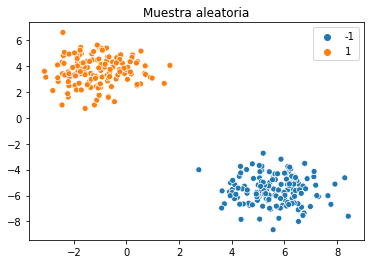
\includegraphics[scale=0.5]{figure/muestra_aleatoria.png}
    \caption{Dataset make$_$blobs}
    \label{fig:muestra_aleatoria}
\end{figure}
Entonces, tenemos que  
\begin{align*}
    \theta(1)=\frac{n}{n_+}=\frac{300}{150}=2, \ \ \ \ \theta(-1)=-\frac{n}{n_-}=-\frac{300}{150}=-2.
\end{align*}
Ahora, procedemos a utilizar la función \textsc{LinearRegression()} para obtener los estimadores por medio de mínimos cuadrados. En donde nuestro vector $Y=[\theta(y_1),\cdots,\theta(y_{300})]$ y la matriz $X$. Los estimadores obtenidos son:
$$\beta_0'=0.76, \ \ \beta=[-0.22274088,  0.26050276]. $$
\textbf{Observando los resultados del clasificador (Ver Figura \ref{fig:fda}), notamos que separa perfectamente las dos categorías de la muestra. Por lo que podemos concluir que es un buen clasificador. }

\begin{figure}[H]
    \centering
    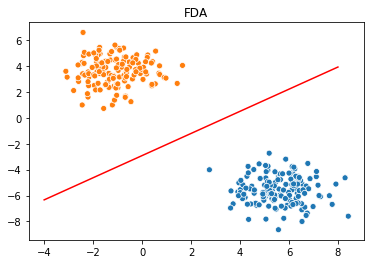
\includegraphics[scale=0.5]{figure/fda.png}
    \caption{Clasificación binaria usando FDA}
    \label{fig:fda}
\end{figure}
\subsection{Ejemplo: Clasificación con datos atípicos}
Nuestro conjunto de datos que utilizamos son la muestra del inciso anterior y generando 5 puntos más en un rango distinto a las dos categorías (datos atípicos). Primero utilizamos mínimos cuadrados para ajustar el clasificador como en la subsección anterior (ver Figura \ref{fig:fda_pesos}). Podemos notar que nuestro clasificador esta muy afectado por nuestros datos atípicos, es decir, podemos notar que FDA no es robusto a datos atípicos.\\  

Para hacer más robusto el clasificador FDA consideramos usar mínimos cuadrados ponderados, es decir, nuestra función de costo a minimizar es
\begin{align*}
\sumi w_i\left(\theta(y_i)-\beta'\xb_i-\beta_0 \right)^2. 
\end{align*}
Donde $w_i$ es un factor de importancia del punto $i$. Nosotros consideramos este factor es inversamente proporcional a la distancia (euclideana) del punto a su centroide de la categoría a la cual pertenece. Es decir,
$$\sqrt{w_i}=\frac{1}{dist(\xb_i, c_{i})}, \ \ \ \ c_{i}\text{ es el centrioide de la categoría de } i.$$
Entonces, para hacer más robustos FDA tenemos que trabajar con los datos: $\Yb_{new}=[\sqrt{w_1}\theta(y_1),\cdots,\sqrt{w_{305}}\theta(y_{305})]$ y $X=\sqrt{w}*X.$ Y los estimadores de mínimos cuadrados se implemente de la misma manera que en la subsección anterior.
\\

Comparando ambas aplicaciones (ver Figura \ref{fig:fda_pesos}), \textbf{podemos observar que con la implementación de mínimos cuadrados ponderados el clasificador binario FDA se vuelve más robusto.}
\begin{figure}[H]
    \centering
    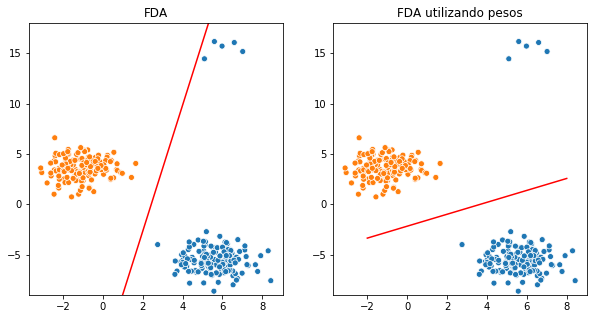
\includegraphics[scale=0.5]{figure/fda_pesos.png}
    \caption{Comparación FDA controlando los datos robustos.}
    \label{fig:fda_pesos}
\end{figure}


\section{Clasificación de MNIST (imágenes de dígitos) }
\subsection{Introducción}
Consideremos los datos \textsc{MNIST} de dígitos escritos a mano de 28 $\times 28$ píxeles. El objetivo es poder clasificar las 70000 imágenes en los dígitos que aparecen en ellas. 


\subsection{Implementación de los distintos métodos  clasificación}
Primeramente partimos nuestro conjunto de datos (imágenes) en dos conjuntos: entrenamiento y prueba. En el conjunto de entrenamiento tenemos 60000 datos y para no tener problemas con una muestra desbalanceada, intentamos en tener una proporción de los dígitos muy parecidas (Ver Cuadro \ref{tab:cont_train}). Lo anterior también se considero para el conjunto de datos de prueba pero en este caso tenemos 10000 datos. \textbf{Debido al tiempo de ejecución de algunos algoritmos utilizados no se considero usar validación cruzada para los ajustes}, pero es un punto muy importante a controlar. 
\begin{table}[H] 
    \centering
    \begin{tabular}{c|c||c|c}
         Dígito& Conteo &Dígito& Conteo \\ \hline \hline
         0  & 5923 & 5  & 5421\\
         1  & 6742 & 6  & 5918\\
         2  & 5958 & 7  & 6265\\
         3  & 6131 & 8  & 5851\\
         4  & 5842 & 9  & 5949 \\ \hline \hline
    \end{tabular}
    \caption{Conteos de los dígitos en los datos de entrenamiento.}
    \label{tab:cont_train}
\end{table}
Todos los métodos se implementaron en python, usando la librería de sklearn (\cite{scikit-learn}).

\subsubsection{Métricas de Evaluación}
Para este ejercicio podríamos considerar solo el \textbf{accuracy} para determinar que tan bueno es el ajuste, ya que se esta utilizando una muestra balanceada. Además de que en este ejercicio no es crucial controlar algún tipo de error especifíco (falsos positivos o verdaderos negativos), como en otros ejercicios por ejemplo referentes a estudios humanos.\\

Pero para tener una mejor perspectiva de los errores consideraremos también las siguientes métricas: \textbf{precisión, recall y F1 score}. 

\subsubsection{Baseline}
Consideraremos como $baseline$ un método de regresión multivariada, es decir, tenemos 
\begin{align*}
    \Yb = \Xb \hat{B},
\end{align*}
donde $\Yb_{n\times |K|}$ es una matriz indicadora, donde cada renglón tiene ceros excepto en lugar que corresponde el valor $y_k$, donde colacamos un 1. $\Xb_{n\times 784}$ es la matriz de características y $\hat{B}$ es la matriz cuyas columnas contienen los $|K|$ coeficientes correspondientes $\hat{\beta}_k.$ Con esta formulación, asumimos un modelo lineal para cada respuesta $y_k:$
\begin{align*}
    \hat{\yb}_k=\Xb\hat{\beta}_k,
\end{align*}
y la clasificación para alguna observación $\xb$ se obtiene mediante 
\begin{align*}
    \hat{C}(\xb)=\arg \max_{k\in K}\hat{y}_k.
\end{align*}
\subsubsection{Resultados Baseline}
Con la sección anterior,   implementamos el método en python al conjunto de entrenamiento y clasificamos las imágenes. Posteriormente calculamos los métricas de error en el conjunto de entrenamiento y prueba, en de entrenamiento para observar si no existe algún sobreajuste en los datos y los errores del conjunto de prueba para contrastar el rendimiento de este modelo con otros modelos (Ver Cuadro \ref{metricas_baseline}).

Comparando el accuracy, precision, recall y f1$-$score de ambos conjunto de datos podemos observar que son muy parecidos, \textbf{por lo que podemos decir que no existe un sobreajuste en los datos}. Concentrándonos en las métricas del conjunto de prueba, podemos observar que en general todos los errores están por arriba de 0.80 a excepción del recall del digíto 2 y 5 (ver Figura \ref{fig:baseline_confusion}). Es decir, en estos dos dígitos nos estamos equivocando en clasificando otros números en 2 y 5. Si observamos \textbf{los f1$-$score y el accuracy podemos notar que todos están por arriba del 0.80, por lo que podemos decir que este modelo tiene un buen rendimiento.}

\begin{table}[H]
    \centering 
    \caption{Métricas de los conjuntos de entrenamiento y prueba.} \label{metricas_baseline}
\begin{minipage}{.5\linewidth}
        \caption{Métricas de entrenamiento}
        \centering
        \begin{tabular}{|c|c|c|c|c}
        \hline
dígito  & precision &  recall & f1-score\\ \hline \hline
0       &     0.90  &  0.96   &  0.93\\  
1       &     0.82  &  0.97   &  0.89\\  
2       &     0.91  &  0.81   &  0.85\\  
3       &     0.84  &  0.84   &  0.84\\  
4       &     0.84  &  0.89   &  0.86\\  
5       &     0.87  &  0.74   &  0.80\\  
6       &     0.89  &  0.93   &  0.91\\  
7       &     0.87  &  0.87   &  0.87\\  
8       &     0.84  &  0.75   &  0.80\\  
9       &     0.81  &  0.80   &  0.81\\ \hline \hline
accuracy  & & & 0.86 \\ \hline \hline
        \end{tabular}
    \end{minipage}%
    \begin{minipage}{.5\linewidth}
      \centering
        \caption{Métricas de prueba}
        \begin{tabular}{|c|c|c|c|c}
        \hline
        dígito  & precision &  recall & f1-score\\
0       &    0.91  &  0.96   &  0.93\\  
1       &    0.83  &  0.98   &  0.90\\  
2       &    0.92  &  0.79   &  0.85\\  
3       &    0.85  &  0.87   &  0.86\\  
4       &    0.81  &  0.90   &  0.85\\  
5       &    0.88  &  0.74   &  0.80\\  
6       &    0.88  &  0.91   &  0.90\\  
7       &    0.85  &  0.86   &  0.86\\  
8       &    0.84  &  0.78   &  0.81\\  
9       &    0.84  &  0.79   &  0.82\\  \hline \hline 
accuracy  & & & 0.86\\ \hline \hline
        \end{tabular}
    \end{minipage} 
\end{table}

\begin{figure}[H]
    \centering
    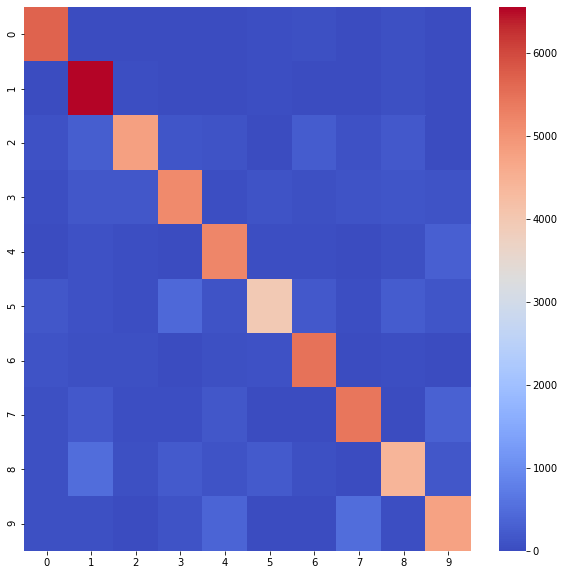
\includegraphics[width=8cm, height=5cm]{figure/baseline_confusion.png}
    \caption{Matriz de confusión del conjunto de prueba.}
    \label{fig:baseline_confusion}
\end{figure}


\textbf{Con las métricas anteriores, intentaremos mejóralas utilizando otros métodos de clasificación: Análisis discriminante lineal (LDA), Análisis discriminante cuadrática (QDA) y Regresión logística.}

\subsubsection{LDA, QDA y Regresión logística}
\textbf{Para este primer acercamiento no consideraremos ninguna transformación o representación de los datos, es decir, simplemente usamos los datos originales.}\\
Primero ocupamos el \textbf{método LDA} y calculamos las métricas de error (ver Cuadro \ref{metricas_lda} y Figura \ref{fig:lda_confusion}). Comparando el accuracy de los dos conjuntos observamos que son muy parecidos, por lo que podemos decir que no existe un sobreajuste. Ahora si comparamos las métricas del conjunto de entrenamiento de este método contra el método $baseline$,  observamos una pequeña mejoría en casi todas las métricas, a excepción de la presición de los dígitos 3, 4, 5 y el recall en los dígitos 1 y 6. Y si comparamos los f1$-$score, en los dígitos 8 y 9 en LDA son menores y en los dígitos restantes son mayores. \textbf{En conclusión, este modelo tiene un mejor rendimiento en comparación con el $baseline$, pero esta diferencia es muy pequeña.}
\begin{table}[H]
    \centering 
    \caption{Métricas de los conjuntos de entrenamiento y prueba, usando LDA.} \label{metricas_lda}
\begin{minipage}{.5\linewidth}
        \caption{Métricas de entrenamiento}
        \centering
        \begin{tabular}{|c|c|c|c|c}
        \hline
dígito  & precision &  recall & f1-score\\
0       &    0.95  &  0.94   &  0.95\\  
1       &    0.87  &  0.96   &  0.91\\  
2       &    0.92  &  0.82   &  0.86\\  
3       &    0.86  &  0.85   &  0.86\\  
4       &    0.86  &  0.90   &  0.88\\  
5       &    0.83  &  0.82   &  0.83\\  
6       &    0.93  &  0.92   &  0.92\\  
7       &    0.92  &  0.84   &  0.88\\  
8       &    0.81  &  0.80   &  0.80\\  
9       &    0.78  &  0.86   &  0.82\\  \hline \hline
accuracy  & & & 0.87\\ \hline \hline
        \end{tabular}
    \end{minipage}%
    \begin{minipage}{.5\linewidth}
      \centering
        \caption{Métricas de prueba}
        \begin{tabular}{|c|c|c|c|c}
        \hline
        dígito  & precision &  recall & f1-score\\
0       &    0.94  &  0.96   &  \textcolor{blue}{0.95}\\  
1       &    0.89  &  0.97   &  \textcolor{blue}{0.93}\\  
2       &    0.92  &  0.79   &  \textcolor{blue}{0.85}\\  
3       &    0.87  &  0.87   &  \textcolor{blue}{0.87}\\  
4       &    0.84  &  0.90   &  \textcolor{blue}{0.87}\\  
5       &    0.84  &  0.82   &  \textcolor{blue}{0.83}\\  
6       &    0.91  &  0.89   &  0.90\\  
7       &    0.91  &  0.84   &  \textcolor{blue}{0.88}\\  
8       &    0.80  &  0.81   &  \textcolor{red}{0.80}\\  
9       &    0.81  &  0.85   &  \textcolor{red}{0.83}\\  \hline \hline
accuracy  & & & \textcolor{blue}{0.87}\\ \hline \hline
        \end{tabular}
    \end{minipage} 
\end{table}
\begin{figure}[H]
    \centering
    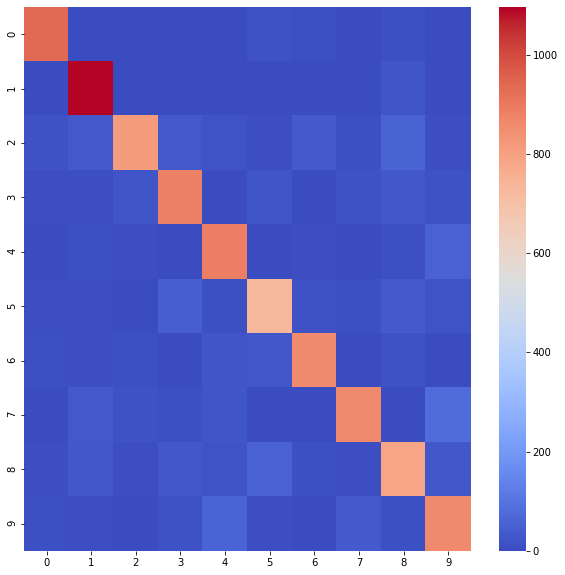
\includegraphics[width=8cm, height=5cm]{figure/lda_confusion.png}
    \caption{Matriz de confusión del conjunto de prueba, usando LDA.}
    \label{fig:lda_confusion}
\end{figure}

Ahora continuemos ocupando \textbf{el método QDA}, realizamos analogamente el análisis anterior. Comparando el accuracy de los dos conjuntos observamos que son muy parecidos, por lo que podemos decir que no existe un sobreajuste. \textbf{Para este modelo no tiene mucho sentido realizar las comparaciones uno a uno, ya que en la mayoría (o todas) las metrícas son peores en este método} (ver Cuadro \ref{metricas_dda}). La razón principal por la cuál no es muy bueno este enfoque es que tal vez las variables que estamos utilizando sean colineales, lo que provoca que la matriz de covarianzas no pueda ser invertible y no converga. Entonces para este método es conveniente reducir el número de variables con PCA o algún otro método.
\begin{table}[H]
    \centering 
    \caption{Métricas de los conjuntos de entrenamiento y prueba, usando QDA.} \label{metricas_dda}
\begin{minipage}{.5\linewidth}
        \caption{Métricas de entrenamiento}
        \centering
        \begin{tabular}{|c|c|c|c|c}
        \hline
dígito  & precision &  recall & f1$-$score\\
0       &    0.37  &  0.98   &  0.54\\  
1       &    0.86  &  0.96   &  0.90\\  
2       &    0.94  &  0.27   &  0.42\\  
3       &    0.70  &  0.39   &  0.51\\  
4       &    0.98  &  0.19   &  0.32\\  
5       &    0.96  &  0.17   &  0.29\\  
6       &    0.70  &  0.98   &  0.82\\  
7       &    0.94  &  0.44   &  0.60\\  
8       &    0.53  &  0.63   &  0.58\\  
9       &    0.50  &  0.96   &  0.66\\  \hline \hline
accuracy  & & & 0.61\\ \hline \hline
        \end{tabular}
    \end{minipage}%
    \begin{minipage}{.5\linewidth}
      \centering
        \caption{Métricas de prueba}
        \begin{tabular}{|c|c|c|c|c}
        \hline
dígito  & precision &  recall & f1$-$score\\
0       &    0.34  &  0.96   &  0.51\\  
1       &    0.89  &  0.95   &  0.92\\  
2       &    0.89  &  0.21   &  0.34\\  
3       &    0.63  &  0.35   &  0.45\\  
4       &    0.95  &  0.16   &  0.27\\  
5       &    0.89  &  0.15   &  0.26\\  
6       &    0.68  &  0.96   &  0.79\\  
7       &    0.92  &  0.39   &  0.55\\  
8       &    0.50  &  0.62   &  0.56\\  
9       &    0.49  &  0.93   &  0.64\\  \hline \hline
accuracy  & & & 0.58\\ \hline \hline
        \end{tabular}
    \end{minipage} 
\end{table}

Y por último, utilizaremos  \textbf{Regresión Logística} para ello realicemos el mismo análisis que los anteriores. En este caso consideraremos dos valores para el parámetro $multi\_class$: $ovr$ y $multinomial$. Usando $ovr$, entonces se ajusta un problema binario para cada etiqueta y para $multinomial$, la pérdida minimizada es el ajuste de pérdida multinomial en toda la distribución de probabilidad, incluso cuando los datos son binarios  (\cite{scikit-learn}). \\

Los métricas con ambos valores del parámetro se observan en el Cuadro \ref{metricas_log_reg} y Figura \ref{fig:log_reg_confusion}. Primero observemos que las diferencias entre los errores del conjunto de datos de entrenamiento y prueba son muy parecidos, por lo que suponemos que no existe sobreajuste. Ahora, considerando las métricas del conjunto de prueba observamos que considerando cualquier valor del parámetro existen pequeñas diferencian en las métricas, pero en general son muy parecidos. \textbf{Si comparamos estas métricas con el método $baseline$ observamos que todas las métricas son mejores,} de hecho en este caso los f1$-$score todos son mayores a 0.89 y el accuary es de 0.93. \textbf{Por lo que, concluimos que este método fue mejor que todos los anteriores (considerando los datos originales, es decir, sin transformaciones ni otra representación).}\\

Y observando la matriz de confusión, podemos notar que el clasificador es muy buen, y que el dígito que más tiene problemas en clasificar es el número 8.

\begin{table}[H]
    \centering 
    \caption{Métricas de los conjuntos de entrenamiento y prueba, usando Regresión Logistica.} \label{metricas_log_reg}
\begin{minipage}{.5\linewidth}
        \caption{Métricas de entrenamiento}
        \centering
        \begin{tabular}{|c|c|c|c|c}
        \hline
dígito  & precision&  recall & f1-score\\
0       &    0.97$-$0.96  &  0.98$-$0.98   &  0.97$-$0.97\\  
1       &    0.97$-$0.96  &  0.98$-$0.98   &  0.97$-$0.97\\  
2       &    0.94$-$0.93  &  0.92$-$0.91   &  0.93$-$0.92\\  
3       &    0.92$-$0.91  &  0.92$-$0.90   &  0.92$-$0.90\\  
4       &    0.95$-$0.93  &  0.95$-$0.94   &  0.95$-$0.93\\  
5       &    0.92$-$0.91  &  0.90$-$0.87   &  0.91$-$0.89\\  
6       &    0.96$-$0.95  &  0.97$-$0.96   &  0.96$-$0.96\\  
7       &    0.95$-$0.94  &  0.95$-$0.94   &  0.95$-$0.94\\  
8       &    0.90$-$0.86  &  0.91$-$0.88   &  0.90$-$0.87\\  
9       &    0.92$-$0.90  &  0.92$-$0.90   &  0.92$-$0.90\\  \hline \hline
accu  & & & 0.94-0.93\\ \hline \hline
        \end{tabular}
    \end{minipage}%
    \begin{minipage}{.5\linewidth}
      \centering
        \caption{Métricas de prueba}
        \begin{tabular}{|c|c|c|c|c}
        \hline
dígito  & precision &  recall & f1$-$score\\
0       &  0.95$-$0.96 &0.98$-$0.98 &  \textcolor{blue}{0.96$-$0.97}\\  
1       &  0.96$-$0.96 &0.98$-$0.98 &  \textcolor{blue}{0.97$-$0.97}\\  
2       &  0.93$-$0.93 &0.90$-$0.91 &  \textcolor{blue}{0.91$-$0.92}\\  
3       &  0.90$-$0.91 &0.92$-$0.90 &  \textcolor{blue}{0.91$-$0.90}\\  
4       &  0.94$-$0.93 &0.93$-$0.94 &  \textcolor{blue}{0.94$-$0.93}\\  
5       &  0.91$-$0.91 &0.86$-$0.87 &  \textcolor{blue}{0.88$-$0.89}\\  
6       &  0.94$-$0.95 &0.95$-$0.96 &  \textcolor{blue}{0.95$-$0.96}\\  
7       &  0.93$-$0.94 &0.92$-$0.94 &  \textcolor{blue}{0.93$-$0.94}\\  
8       &  0.87$-$0.86 &0.89$-$0.88 &  \textcolor{blue}{0.88$-$0.87}\\  
9       &  0.91$-$0.90 &0.92$-$0.90 &  \textcolor{blue}{0.91$-$0.90}\\  \hline \hline
accu  & & & \textcolor{blue}{0.93-0.93}\\ \hline \hline
        \end{tabular}
    \end{minipage} 
\end{table}
\begin{figure}[!htb]
\minipage{0.4\textwidth}
  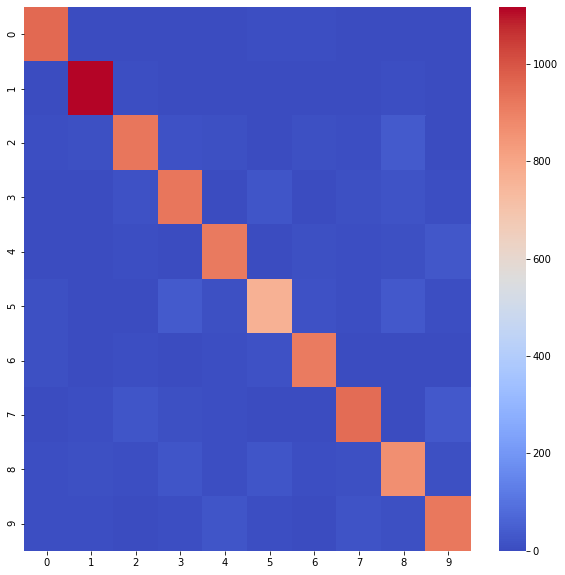
\includegraphics[width=\linewidth]{figure/log_reg_confusion.png}
\endminipage\hfill
\minipage{0.4\textwidth}
  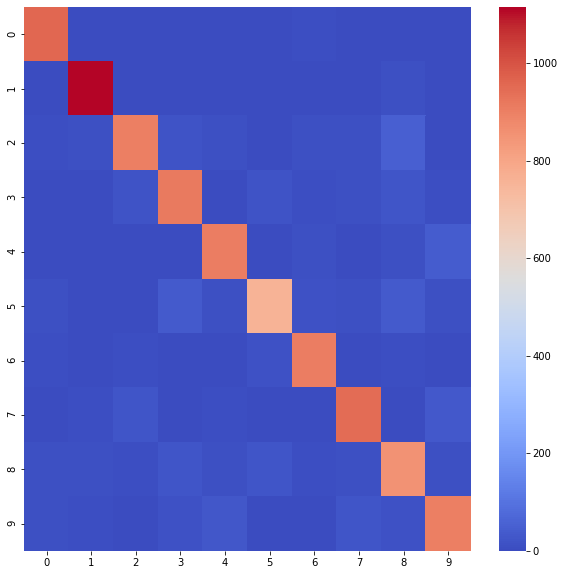
\includegraphics[width=\linewidth]{figure/log_reg2_confusion.png}
\endminipage
\caption{Matriz de confusión del conjunto de prueba, usando Reg Log.}
\label{fig:log_reg_confusion}
\end{figure}

\subsection{Nueva representación de los datos.}
Para este caso no se considera una estandarización o escalamiento de los datos, debido a que los métodos LDA, QDA y Regresión Logística son robustos a estas transformaciones.\\

El siguiente paso a considerar fue reducir la dimensionalidad. \textbf{Debido a que tenemos alrededor de 800 variables, posiblemente existan variables que no sean relevantes (exista una alta correlación). Por lo cual, consideramos utilizar PCA para reducir el número de variables.} Los métodos LDA y Regresión Logística tuvieron pequeños cambios, \textbf{pero QDA} (que si recordamos era el método que presentaba los peores errores de este ejercicio) \textbf{presento un cambio muy significativo, al grado de ser el método con las mejores métricas. }

\subsubsection{Comparación de métricas: QDA y Regresión Logística}

Primeramente \textbf{utilizamos PCA para reducir el número de variables a 200 de nuestro conjunto de datos de entrenamiento} (no probé con distintos valores de número de componentes). Posteriormente proyectamos nuestro conjunto de prueba con los valores del PCA ajustado. Y finalmente \textbf{utilizamos QDA para clasificar las imágenes}. \\

Comparando con las métricas de QDA y las que obtuvimos anteriormente de los modelos de Regresión Logística, los f1$-$score en la mayoría de los casos están por arriba o igual que el mejor modelo de Regresión Logística (ver Cuadro \ref{metricas_qda_bst} y Figura \ref{fig:comparacion_bbst}). 
El dígito 8 es el que presenta más error de clasificación, \textbf{pero en general podrías concluir que este ajuste es el mejor que todos los que se probaron.}


\begin{table}[H]
    \centering 
    \caption{Comparación de metricas en el conjunto de entrenamiento: Reg Log y QDA.} \label{metricas_qda_bst}
\begin{minipage}{.5\linewidth}
        \caption{Métricas usando Reg Log}
        \centering
        \begin{tabular}{|c|c|c|c|c}
        \hline
dígito  & precision &  recall & f1$-$score\\
0       &   0.95  &  0.98   & 0.96\\  
1       &   0.96  &  0.98   & 0.97\\  
2       &   0.93  &  0.90   & 0.91\\  
3       &   0.90  &  0.92   & 0.91\\  
4       &   0.94  &  0.93   & 0.94\\  
5       &   0.91  &  0.86   & 0.88\\  
6       &   0.94  &  0.95   & 0.95\\  
7       &   0.93  &  0.92   & 0.93\\  
8       &   0.87  &  0.89   & 0.88\\  
9       &   0.91  &  0.92   & 0.91\\  \hline \hline
accuracy  & & & 0.93\\ \hline \hline
        \end{tabular}
    \end{minipage}%
    \begin{minipage}{.5\linewidth}
      \centering
        \caption{Métricas usando QDA}
        \begin{tabular}{|c|c|c|c|c}
        \hline
dígito  & precision &  recall & f1$-$score\\
0       &   0.97  &  0.98   & \textcolor{blue}{0.98}\\  
1       &   0.99  &  0.95   & 0.97\\  
2       &   0.93  &  0.96   & \textcolor{blue}{0.94}\\  
3       &   0.94  &  0.92   & \textcolor{blue}{0.93}\\  
4       &   0.96  &  0.96   & \textcolor{blue}{0.96}\\  
5       &   0.95  &  0.91   & \textcolor{blue}{0.93}\\  
6       &   0.97  &  0.95   & 0.96\\  
7       &   0.97  &  0.93   & \textcolor{blue}{0.95}\\  
8       &   0.83  &  0.95   & 0.88\\  
9       &   0.94  &  0.93   & \textcolor{blue}{0.93}\\  \hline \hline
accuracy  & & & \textcolor{blue}{0.94}\\ \hline \hline
        \end{tabular}
    \end{minipage} 
\end{table}
\begin{figure}[!htb]
\minipage{0.4\textwidth}
  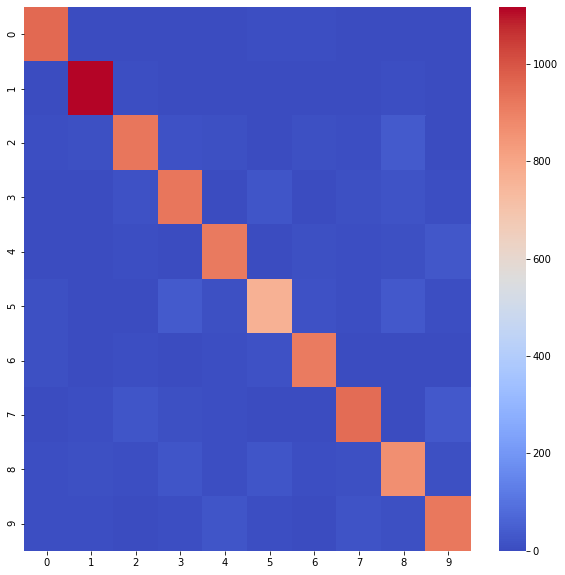
\includegraphics[width=\linewidth]{figure/log_reg_confusion.png}
\endminipage\hfill
\minipage{0.4\textwidth}
  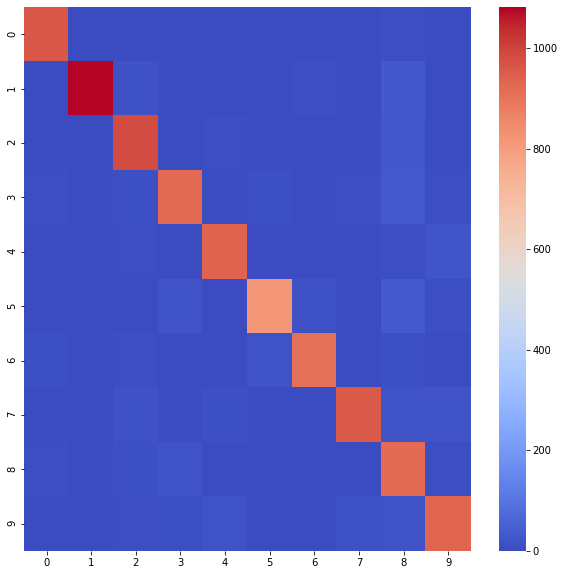
\includegraphics[width=\linewidth]{figure/qda_confusion_best.png}
\endminipage
\caption{Matriz de confusión del conjunto de prueba, usando Reg Log y QDA}
\label{fig:comparacion_bbst}
\end{figure}
Podemos concluir, que tenemos que tener cuidado con los métodos QDA y LDA ya que estos tienen supuestos que deben de cumplir para tener un mejor rendimiento. Claramente se pudo observar este efecto en este ejercicio.


\section{Análisis de texto y de sentimientos.}
Tenemos 400 opiniones de usuarios tanto positivas como negativas acerca de los siguientes productos: automóviles, hoteles, lavadoras, libros, teléfonos celulares, música, computadoras y películas.

\subsection{Bad of Words (BOW)}
Antes a realizar algún análisis con los datos, tenemos que realizar un preproceso y normalización del texto. Nosotros realizamos lo siguiente:
\begin{enumerate}
    \item Convertimos todas las letras a minúsculas.
    \item Eliminamos signos de puntuación, acentos y otros signos diacríticos.
    \item Eliminamos caracteres repetidos (ejemplo: taaaaanto), saltos de línea y espacios en blanco.
    \item Eliminamos palabra funcionales (stop words).
    \item Y por último, aplicamos stemming y lematización. 
\end{enumerate}
Lo anterior se realizo debido a que las opiniones estaban muy , lo que provocaría un sesgo. Se probó con diferentes combinaciones, pero el conjunto de datos que presentaba mejores resultados fue cuando se realizaron las anteriores tareas de limpieza.\\

Además, consideremos diferentes valores para tamaño de vocabulario. Nos dimos cuenta que entre más pequeño sea el tamaño del vocabulario existe una mayor cantidad de opiniones con distancias cercanas a 1, en cambio cuando el tamaño era demasiado grande las distancias eran muy cercanas a 0. Es decir, lo anterior tiene mucho sentido debido a que la distancia esta muy relacionada con las palabras que se usaran en el vocabulario. Seleccionamos el tamaño de vocabulario observando la matriz de distancias, \textbf{ya que con un valor de $V=3000$ es sencillo identificar de forma visual los grupos de opiniones de productos y sentimientos.}\\

Y por último, otro factor a considerar es el \textbf{rango de n$-$valores para diferentes n$-$gramas de palabras.} Probamos con diferentes rangos, pero si el rango era grande la interpretación de las distancias era complicada. Y si el valor era grande, la información era mínima. \textbf{Por lo cuál solo consideremos una palabra, es decir, el rango fue de $(1,1)$.}

\subsection{Matriz de similaridades usando BOW y la distancia coseno.}
Con la representación BOW descrito en la sección anterior, procedemos a calcular la matriz de similaridades considerando la distancia coseno:
$$k(x,y)=\frac{xy^T}{||x||||y||}.$$

Si ordenamos las opiniones de por el número de artículos, y comparando la matriz de distancias de las opiniones con una matriz de distancias realizadas solo con la palabra del artículo a que opinan (ver Figura \ref{fig:productos_distancia}), es decir, queremos contrastar si podemos reconocer las opiniones según los productos calificados. Comparando estas dos matrices de distancias, podemos observar claramente el patrón de los productos en las opiniones.

\begin{figure}[!htb]
\minipage{0.4\textwidth}
\caption{Matriz de distancias de las opiniones.}
  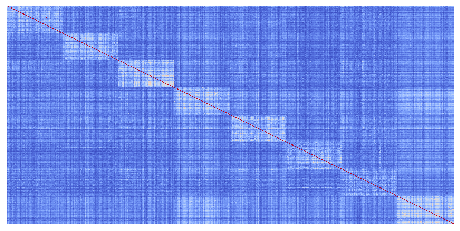
\includegraphics[width=\linewidth]{figure/bow_productos_distancia.png}
\endminipage\hfill
\minipage{0.4\textwidth}
\caption{Matriz de distancias del vector de productos.}
  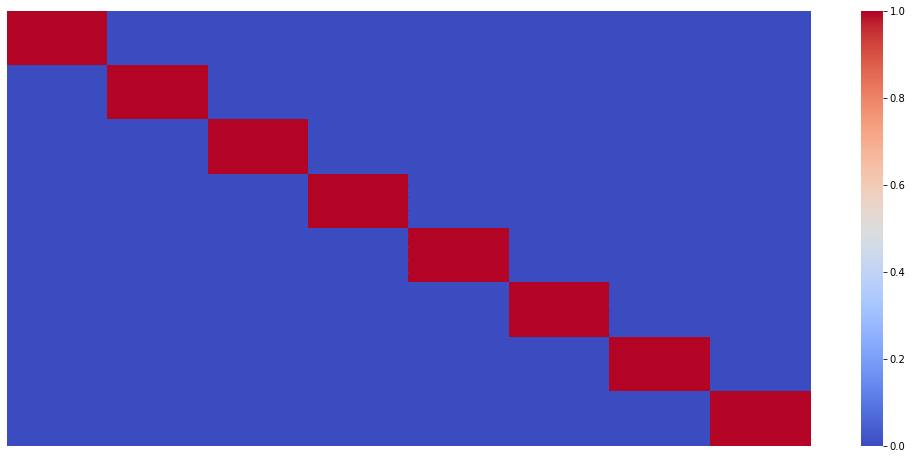
\includegraphics[width=\linewidth]{figure/productos_distancia.png}
\endminipage
\caption{Reconocimiento visual de patrones de los productos en las opiniones.}
\label{fig:productos_distancia}
\end{figure}

Ahora realicemos un nuevo ordenamiento para comparar la matriz de distancias de las opiniones y con una matriz de considerando un vector compuestas de 400 registros cada uno con los productos y sentimiento (ver Figura \ref{fig:productos_sentimientos_distancia}). Para este caso, \textbf{se observa un poco el patrón de los segmentos de los productos y sentimientos de las opiniones, claramente no es para todas las combinaciones pero si es un buen proxy de segmentación.}
\begin{figure}[!htb]
\minipage{0.4\textwidth}
\caption{Matriz de distancias de las opiniones.}
  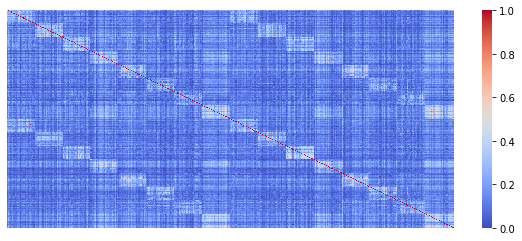
\includegraphics[width=\linewidth]{figure/bow_productos_sentimientos.png}
\endminipage\hfill
\minipage{0.4\textwidth}
\caption{Matriz de distancias del vector de productos y sentimientos..}
  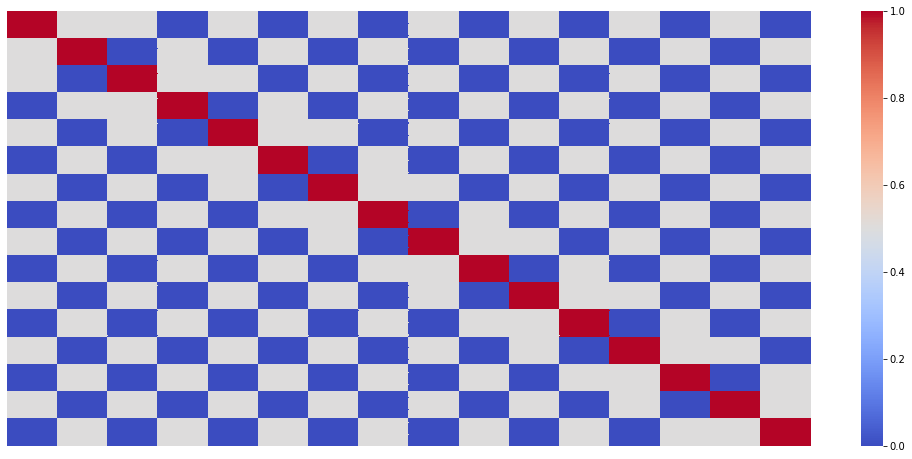
\includegraphics[width=\linewidth]{figure/productos_sentimientos_distancia.png}
\endminipage
\caption{Reconocimiento visual de patrones de los productos y sentimientos en las opiniones.}
\label{fig:productos_sentimientos_distancia}
\end{figure}


\subsection{Clustering en las representaciones BOW.}
Usando la matriz de similaridades calculada en el sección anterior, procedemos a implementar distintos métodos de clustering (KMeans, Kernel KMeasn, Spectral Clustering) para encontrar las opiniones a partir de los productos que evaluaban y el sentimiento de la opinión (positiva o negativa).\\

Para presentar \textbf{los resultados procedimos primero representar la representación BOW en dos dimensiones, con el objetivo de observar visualmente los clustering.} Probamos distintos métodos de reducción de dimensionalidad (PCA, KPCA, TSN$-$E y SE). \textbf{La mejor representación fue considerando Spectral Embedding ($gamma=0.6$ y $n\_neigbors=10$)} (ver Figura \ref{fig:BOW_2D}). \\
\textbf{Debido a que tenemos las categorías de las opiniones podemos validar de forma cuantitativa los clusters encontrados.} En la vida real cuando clustering no supervisado esto no es posible, pero para fundamentar mejor las visualizaciones de este análisis utilizamos las métricas de para un ajuste de clasificación.
\begin{figure}[H]
    \centering
    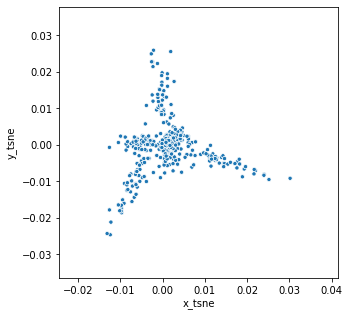
\includegraphics[scale=0.6]{figure/BOW_2D.png}
    \caption{Representación 2D usando SE}
    \label{fig:BOW_2D}
\end{figure}
\textbf{El mejor modelo que encuentra algunos patrones interesantes fue utilizando Spectral Embedding Clustering.} Primero intentamos encontrar las opiniones de acuerdo a los sentimientos, para ello consideramos buscar dos clustering en nuestro método (ver Figura \ref{fig:BOW_sentimientos_2D}). En este caso no pudimos encontrar las categorías esperadas de los sentimientos ($yes,\ no$), de hecho si comparamos con las clasificaciónes reales el accuracy final sería de 0.52. Lo cual nos puede indicar que nuestros clusters no es buena para encontrar los sentimientos.

\begin{figure}[H]
    \centering
    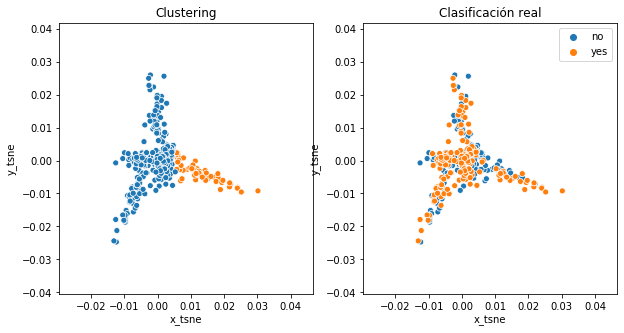
\includegraphics[scale=0.7]{figure/BOW_sentimientos_2D.png}
    \caption{Clustering para los sentimientos}
    \label{fig:BOW_sentimientos_2D}
\end{figure}
Ahora, si buscamos 8 categorías en nuestro conjunto de datos obtenemos los 8 clusters que se ven en la Figura \ref{fig:BOW_productos_2D}. Si comparamos los clustering encontrados con las categorías reales obtenemos un accuracy del 0.94, además de que las métricas de precisión, recall y f1$-$score son buenas. Es decir, \textbf{este modelo pudo identificar perfectamente las categorías de los productos en las opiniones}. 
\begin{figure}[H]
    \centering
    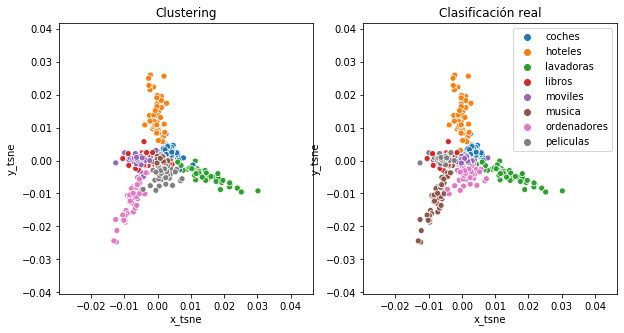
\includegraphics[scale=0.7]{figure/BOW_productos_2D.png}
    \caption{Clustering para los productos}
    \label{fig:BOW_productos_2D}
\end{figure}
Por último, intentamos encontrar las opiniones para cada producto y por sentimiento. En total son 16 categorías diferentes, pero en general no pudimos encontrar todas estas categorías. 
\begin{figure}[H]
    \centering
    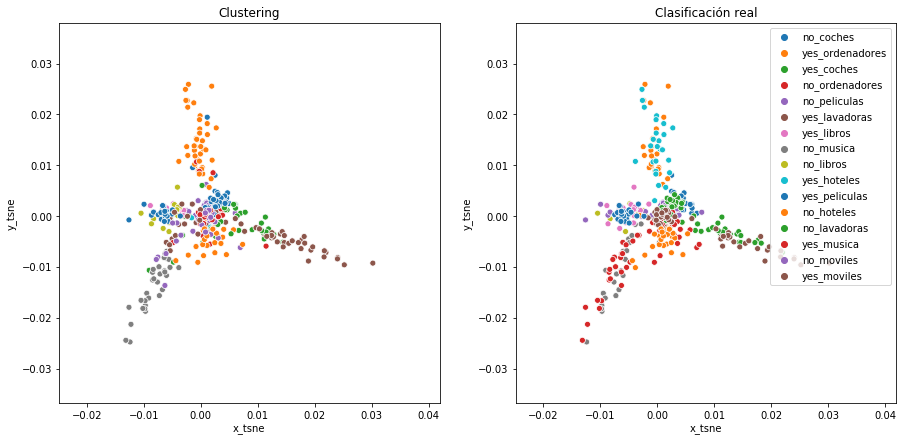
\includegraphics[scale=0.5]{figure/BOW_productos_sentimientos_2D.png}
    \caption{Clustering para los sentimientos y productos}
    \label{fig:BOW_productos_sentimientos_2D}
\end{figure}
Algo interesante a observar es que hay ciertas categorías de productos y sentimientos que si se pueden identificar muy bien (lavadoras con el sentimiento \textit{yes}, o hoteles con los sentimientos \textit{no}), hay otras combinaciones que en las cuales se confunden con los sentimientos. Por ejemplo, las opiniones que hablan de los coches no es posible separar los sentimientos: \textit{yes y no}.
\begin{figure}[H]
    \centering
    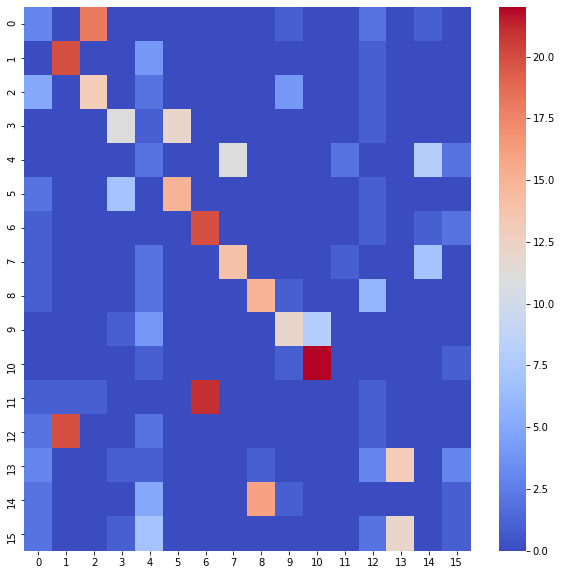
\includegraphics[scale=0.3]{figure/heatmap_productos_sentimientos.png}
    \caption{Matriz de confusión de las opiniones considerando los sentimientos y productos}
    \label{fig:my_label}
\end{figure}
Por lo anterior, \textbf{podemos concluir que es posible identificar las opiniones por productos pero no es posible identificar por sus sentimientos. Y cuando se intentar identificar las opiniones por productos y sentimientos, la mayoría de las combinaciones no es posible identificarlas ya que se confunden con sus respectivas opiniones pero con distinto sentimientos.}

\subsection{Clasificación supervisada de las opiniones respecto a los sentimientos y productos.}

El objetivo de esta subsección fue poder clasificar las opiniones conforme a los productos y sentimientos, mediante un modelo supervisado. \\

Para ello primero partimos nuestro conjunto de datos en dos conjuntos ($70-30$): entrenamiento y prueba. \textbf{En el conjunto de entrenamiento consideramos varios modelos con diferentes valores en sus parámetros y además diferentes representación de los datos}. Los modelos ocupados fueron \textbf{LDA, QDA y Regresión logística, las representaciones de los datos consideradas fue la reducción de dimensionalidad de las variables usando PCA donde probamos diferentes número de componentes principales}. Y por último, en el modelo de regresión logística utilizamos \textbf{regularización $l2$} debido a que teníamos un problema de sobreajuste, consideramos diferentes valores de regularización: 0.1, 0.05, 0.0094, 0.005. Para el modelo de regresión logística ocupamos \textbf{validación cruzada (cv=9)} para controlar el sobreajuste de los datos, solo se realizo en este modelo debido a que en la librería de sklearn ya viene una implementación de este modelo usando CV.


\subsubsection{Clasificación de los sentimientos}
Empecemos presentando los resultados de los modelos para poder predecir el sentimiento a partir de los sentimientos. Los modelos \textbf{LDA y QDA} tienen un muy buen rendimiento cuando se usan una mayor cantidad de componentes principales en el conjunto de entrenamiento. P\textbf{ero el principal problema de estos modelos fue que sobreajustaron} a los datos, ya que al calcular las métricas de error en el conjunto de prueba estas eran muy malas. Por ejemplo, \textbf{usando LDA con 200 componentes principales el accuracy en el conjunto de entrenamiento es de 0.96. En cambio el accuracy en el conjunto de prueba es de 0.58, lo que implica que hay un sobreajuste en los datos.} \\

Ahora, \textbf{utilizando Regresión logística la mejor combinación fue ocupando una penalización de 0.005 y 200 componentes principales} (ver Cuadro \ref{metricas_reviews}). Cabe mencionar que existe una gran diferencia en las métricas del conjunto de entrenamiento y prueba, pero como se utilizo validación cruzada para estos resultados se cree que están mejor fundamentados. 
\begin{table}[H]
    \centering 
    \caption{Comparación de métricas en el conjunto de entrenamiento y prueba, Reg Log.} \label{metricas_reviews}
\begin{minipage}{.5\linewidth}
        \caption{Conjunto de entrenamiento}
        \centering
        \begin{tabular}{|c|c|c|c|c}
        \hline
review  & precisión &  recall & f1$-$score\\
yes     &   0.99  &  0.98   & 0.99\\  
no      &   0.98  &  0.99   & 0.98\\  \hline \hline
accuracy  & & & 0.99\\ \hline \hline
        \end{tabular}
    \end{minipage}%
    \begin{minipage}{.5\linewidth}
      \centering
        \caption{Conjunto de prueba}
        \begin{tabular}{|c|c|c|c|c}
        \hline
review  & precisión &  recall & f1$-$score\\
yes     &   0.74  &  0.65   & 0.69\\  
no      &   0.69  &  0.77   & 0.72\\  \hline \hline
accuracy  & & & 0.71\\ \hline \hline
        \end{tabular}
    \end{minipage} 
\end{table}

\subsubsection{Clasificación de los productos}
Para predecir de que producto están hablando a partir de las opiniones realizamos lo mismo que en las subsecciones anteriores. Para este caso, los modelos probados de QDA fueron los que presentaron peores métricas, debido a que se sobreajustaban bastante al conjunto de entrenamiento. Esto puede deberse a que este modelo no es robusto a valores extremos, lo que provoca un mal rendimiento en el conjunto de prueba. De igual manera se observa con los modelos de LDA, pero este hecho es menos notorio.\\

\textbf{El mejor modelo es considerar ocupar regresión logística ocupando una regularización de 0.01 en los primeros 200 componentes principales} (ver Cuadro \ref{metricas_producto}). Las métricas la mayoría están muy cercanas a 1, lo que pudiera indicar un problema de sobreajuste pero debido a que se utilizo validación cruzada descartamos esta opción.
\begin{table}[H]
    \centering 
    \caption{Comparación de métricas en el conjunto de entrenamiento y prueba, Reg Log.} \label{metricas_producto}
\begin{minipage}{.5\linewidth}
        \caption{Conjunto de entrenamiento}
        \centering
        \begin{tabular}{|c|c|c|c|c}
        \hline
producto  & precisión &  recall & f1$-$score\\
      coches & 1.00 &1.00 &1.00\\    
     hoteles & 1.00 &1.00 &1.00\\    
   lavadoras & 1.00 &1.00 &1.00\\
      libros & 1.00 &1.00 &1.00\\
     moviles & 1.00 &0.97 &0.98\\
      musica & 0.97 &1.00 &0.98\\
 ordenadores & 0.97 &1.00 &0.98\\
   peliculas & 1.00 &0.97 &0.99\\ \hline \hline
accuracy  & & & 0.99\\ \hline \hline
        \end{tabular}
    \end{minipage}%
    \begin{minipage}{.5\linewidth}
      \centering
        \caption{Conjunto de prueba}
        \begin{tabular}{|c|c|c|c|c}
        \hline
review  & precisión &  recall & f1$-$score\\
      coches & 1.00 &1.00 &1.00\\    
     hoteles & 1.00 &1.00 &1.00\\    
   lavadoras & 1.00 &1.00 &1.00\\
      libros & 1.00 &0.91 &0.95\\
     moviles & 1.00 &0.94 &0.97\\
      musica & 1.00 &1.00 &1.00\\
 ordenadores & 0.95 &1.00 &0.97\\
   peliculas & 0.92 &1.00 &0.96\\ \hline \hline
accuracy  & & & 0.98\\ \hline \hline
        \end{tabular}
    \end{minipage} 
\end{table}


\subsection{Conclusión}
Por un lado \textbf{podemos concluir que fue sencillo encontrar y predecir los patrones de los productos en las opiniones. Pero poder identificar si las opiniones eran positivas o negativas resulto un poco más complicado}, tal vez se deba a la limpieza del texto. Estaría interesante ver el efecto de una representación de BOW solo usando palabras que nos den indicios de disgusto o agradecimiento, es decir, considerar palabras muy especificas: gracias, excelente, pésimo, maravilloso, etc. \\

Y por otro lado, nos dimos cuenta de lo sensible que son los modelos. Es decir, realizar las tareas de validación cruzada, separar nuestro conjunto de entrenamiento y prueba nos ayuda a no cometer errores de sobreajuste. Además, los modelos de \textbf{LDA y QDA} son muy sensibles a valores extremos lo que hace que los errores aumenten en un conjunto de datos distinto al de entrenamiento. 




\section{Anexos}
Todos los códigos utilizados para estos resultados se pueden encontrar en mi página personal de Gitgub: Enriquesec. En el repositorio Ciencia de Datos/Tareas/Tareas$_$5/.


\printbibliography




\end{document}